\documentclass{article}
\usepackage{nips15submit_e}
\usepackage{graphicx}
\usepackage{caption}
\usepackage{listings}
\usepackage{color}

\definecolor{codegreen}{rgb}{0,0.6,0}
\definecolor{codegray}{rgb}{0.5,0.5,0.5}
\definecolor{codepurple}{rgb}{0.58,0,0.82}
\definecolor{backcolour}{rgb}{0.95,0.95,0.92}

\lstdefinestyle{mystyle}{
    backgroundcolor=\color{backcolour},
    commentstyle=\color{codegreen},
    keywordstyle=\color{magenta},
    numberstyle=\tiny\color{codegray},
    stringstyle=\color{codepurple},
    basicstyle=\footnotesize,
    breakatwhitespace=false,
    breaklines=true,
    captionpos=b,
    keepspaces=true,
    numbers=left,
    numbersep=5pt,
    showspaces=false,
    showstringspaces=false,
    showtabs=false,
    tabsize=2
}

\lstset{style=mystyle}

\begin{document}
\title{Porting the Jacobi Code to OpenMP \\
{\large Introduction to High Performance Computing COMS30005}}
\maketitle

\section{Introduction}
The trend in modern HPC is clear: parallelization is the way
forward. In every aspect, performance is being found through
concurrent execution; be that via vectorisation, multi-core CPUs or
even GPGPU computing. Despite programming challenges arising from this
new paradigm, the benefits on offer make it more than worth the
effort.

To illustrate the potential performance gains on offer, what follows
is a walkthrough of a successful attempt to parallelize optimised
serial code running the Jacobi algorithm for solving a set of linear
equations, by porting it to OpenMP.

\subsection{Methodology} After making a change, the program was
re-profiled and the new run-time for matrices of orders 500, 1000,
2000 and 4000 recorded, averaged and rounded to an appropriate
accuracy across three runs on BlueCrystal. Times are given in the
format W/X/Y/Z for each matrix order respectively and are in
seconds. For convenience, where significant performance gains were
made, improvements are described in terms of ``\(t\)X times faster''
(where \(t\) is the speedup); whereas smaller improvements are
described in terms of percentages.

\subsection{Serial Optimisations}
Prior to parallelization, a number of basic changes and optimisations
of the serial code were explored. In order of implementation, with
performance gain relative to the preceeding optimisation's times,
these were:

\begin{enumerate}
\item Change compiler from GNU (gcc 4.8.5) to Intel (icc 18.0.0): \textbf{\~3X
  faster}
\item Ensure data order and data access pattern are the same (column
  vs. row traversal): \textbf{\~3.5X faster}
\item Change data type from \texttt{double} to \texttt{float}:
  \textbf{\~5\%-10\% faster}
\item Enable \texttt{-O3} compiler optimisation flag: \textbf{\~15\% faster}
\item Vectorisation check using \texttt{-qopt-report}
\end{enumerate}

These optimisations resulted in runtimes at submission of
0.148/1.107/7.879/72.155 (down from approximately 1.5/10/130/1180 for
unoptimised code).

\subsubsection{Further Serial Optimisations}
In addition to the above, one further optimisation became apparent
after submission and was dutifully included in the serial code before
embarking on this parallelization endeavour. The branching code
\texttt{if (row != col)} in the \texttt{run()} method was removed
entirely and instead, a looping technique that avoids irerating on
that particular matrix element altogether was employed, thus better
facilitating pipelining and vectorisation.

\section{Parallelisation}

\subsection{Baseline}
To judge relative performance improvements, a baseline runtime is
required. The serial code with the above optimisations and changes
from the first submission (continuing with \texttt{icc} and
\texttt{-O3} optimisation), including the one further optimisation,
produced runtimes of 0.137/0.994/6.891/66.731.

\subsection{Performance Analysis}
Relative performance improvements are good, but how does a programmer
know if he is really running fast code? What exactly is ``fast''?
Measuring absolute performance gains against a theoretical maximum
performance can help answer this. The concept of ``operational
intensity'' can be used to produce a few illustrations of
theoretical maximum performance.

\subsubsection{Computational Complexity}
It is useful to first understand the computational complexity (CC) of
the Jacobi code in terms of ``big O'' notation. The key part of the
Jacobi algorithm processes a matrix, nesting two adjacent \texttt{for}
loops that process matrix columns inside another \texttt{for} loop,
processing each row:

\begin{lstlisting}[language=C]
// Perform Jacobi iteration
for (row = 0; row < N; row++)
{
  dot = 0.0;
  skip_count = N;

  for (col = 0; col < row; col++)
  {
    dot += A[row*N + col] * x[col];
  }
  // Skip matrix element where col==row
  for (col = (row + 1); col < N; col++)
  {
    dot += A[row*N + col] * x[col];
  }

  xtmp[row] = (b[row] - dot) / A[row*N + row];
}
\end{lstlisting}

If each of these loops takes \(O(n)\) where \(n\) is the matrix
order, then the CC is \(O(n^2)\). This means the computational
requirement scales exponentially with the size of the matrix order.

\subsubsection{Operational Intensity}
Whereas CC only accounts for compute cost, operational intensity (OI)
can describe the relationship between compute and memory cost. This is
a measure that can be described as ``operations per byte of memory
traffic''.

By simply looking at the solver portion of the Jacobi code, we can
identify the memory operations required during matrix
processing. Working through the code block systematically, there are 8
bytes loaded/stored, and there are 2 operations executed, giving an OI
of 2/8 or 0.25.

\subsubsection{STREAM Benchmark}
Another way of measuring absolute performance is with the STREAM
benchmark. This measures the peak sustainable memory bandwidth on
specific hardware. Knowing the result of this benchmark for
BlueCrystal can tell us how close we are to achieving peak memory
bandwidth.

STREAM benchmark results available from Simon McIntosh-Smith for an
Intel Xeon CPU E5-2670 (SB) 8-cores gave the following results:

\begin{center}
  \begin{tabular}{|l|l|}
    \hline
    \textbf{Memory Level} & \textbf{Bandwidth in GB/s} \\
    L1 cache & 776 \\
    L2 cache & 390 \\
    L3 cache & 209 \\
    DRAM & 34.4 \\
    \hline
  \end{tabular}
\end{center}

\subsubsection{Roofline Model}
Now the OI and peak memory bandwidth can be used in a roofline
model. This graph provides a visual means of identifying optimal
performance in terms of a trade-off between compute and memory
cost. We can also identify where the code is under the ``roof'' of the
graph, to determine whether the code is compute-bound or memory-bound,
helping to focus optimisation and parallelization efforts.

\begin{figure}
\captionsetup{justification=centering}
\centering
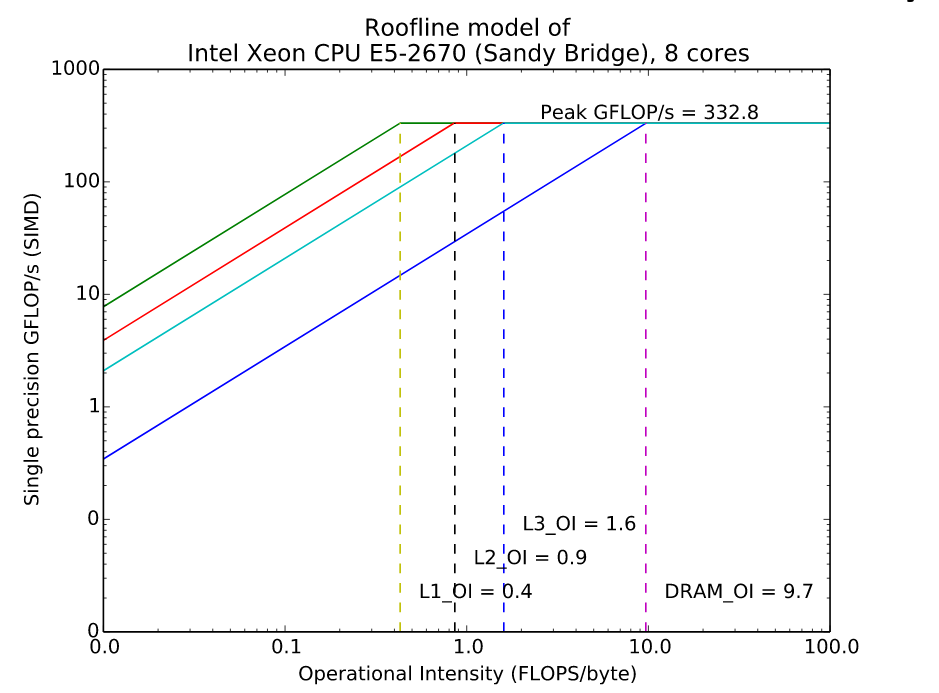
\includegraphics[scale=0.4]{roofline}
\caption{Cache-aware roofline model for a BCP3 CPU}
\end{figure}

Figure 1 shows a cache-aware roofline model for a BlueCrystal
CPU. Taking the Jacobi OI of 0.25, it is clear this figure lies way
below the peak performance point with reference to DRAM. However it is
not particularly far from the peak performance mark of the L1
cache. If code modifications took place and the Jacobi OI became above
0.4, and if the code was hitting the L1 cache the majority of the
time, this figure would become relevant because then, the code would
change to be compute bound!

\subsection{Adding Pragmas}
Now on to the parallelisation itself. The most obvious thing to do
initially is to turn the \texttt{for} loops into parallel \texttt{for}
loops. This can be done with the pragma \ldots

Several loops are available for parallelisation: \ldots

\subsection{Profiling}
To check the results of adding these OpenMP pragmas, profiling is
necessary to get a better idea of exactly what the code is
doing. \texttt{Tau} is a good profiler for multi-threaded code. The
\texttt{Tau} output for the code after a quick and dirty
parallelisation is:

\ldots

gperftools?

\subsection{Cache coherency/false sharing}
Reduction

\subsection{Reprofiling}
After the above cleaning up the parallelisation, the code was
re-profiled and the runtimes were now W/X/Y/Z.

Now is a good time to mention the overhead of parallelisation. Clearly
the run times have not been decreasing in a direct relationship with
the increasing number of cores (i.e. when using 4 cores instead of 1,
the code is not 4 times faster). This is because parallelisation of
code introduces some overhead with regards to thread
management. Because the code is now more complex and things like
memory conflicts and thread lifecycles must be managed, the
performance gain is not directly related to the increase in processing power.

\subsection{Libraries}
According to the ``seven dwarves'' paper, the vast
majority of code executed in HPC falls into one of seven
categories. This concept is useful because knwoing which of the
``dwarves'' a piece of code is, may mean that historically, similar
code has been dealt with before. Looking at these past examples may
provide help on how to better solve your problem.

The Jacobi solver falls into the ``dense linear algebra''
category. From research, the BLAS and NAG C libraries are applicable
to this category of HPC. These libraries contain many common mathematical
functions, written in a highly optimised manner - for example, matrix
manipulation. These libraries were tested in the parallel code where
appropriate, and the resulting times after swapping home-grown code
for the library code was W/X/Y/Z.

\subsection{Re-testing compiler}
Compiler optimisations can be somewhat of a mystery. The complexity of
modern compilers means their behaviour is not always predictable in
advance. Sometimes, less agressive optimisation flags can be faster
than more aggressive flags, for example.

Testing of the following compiler flags was undertaken after
parallelisation to check behaviour:

\begin{itemize}
\item Optimisation flags \texttt{-O, -O2, -O3}: 
\item 
\end{itemize}

\section{Conclusion}
Overall,

\subsection{Going Further}
In terms of further optimisation, loop fusion was attempted in the
Jacobi solver, to combine matrix processing with convergence
check. However this introduced a high error rate (probably
bug). Successfully implementing this could realise further performance
gains.

One final useful thing to know is how well a piece of code will scale
with further parallelization. Testing the Jacobi algorithm on a
growing number of cores results in the following graph:

\ldots

Which means the scaling is type\ldots

So can be scaled more/cannot be scaled that well

Amdahl's Law Gustavson's Law

\end{document} 